\section{Building OpenWebMath}

\subsection{Objectives}

Our aim with OpenWebMath is to build a dataset of as many mathematical documents sourced from the web as possible while preserving the formatting of mathematical content such as \LaTeX{} equations as in \citet{lewkowycz2022solving}. For the purposes of this work, we define a mathematical document as a document containing either core mathematical contents such as theorems, definitions, proofs, questions and answers, formal mathematics, or interdisciplinary documents featuring mathematical formulas within fields like physics, chemistry, biology, economics, and finance. We source our documents from Common Crawl, which is a large open-access crawl of the web containing petabytes of raw HTML files. Due to the high variance in the quality of documents from Common Crawl, we additionally use several methods for filtering and boilerplate reduction. Throughout the creation of OpenWebMath, we iteratively refined these methods to ensure that we do not remove too many relevant documents, optimizing for high recall whenever possible. Since we expect that OpenWebMath will be used primarily as an additional source of pretraining data for large language models, we prefer having a small percentage of non-mathematical but high quality documents in the dataset rather than removing them and potentially losing relevant mathematical content. Finally, due to the limited number of mathematical data available on the web, we use significantly more manual inspection and tuning of our processing pipeline than other web-based datasets. We document our processing choices and pipeline in the section that follows.

\subsection{High-level overview of the pipeline}



As shown in \autoref{fig:pipeline}, the processing pipeline for OpenWebMath falls into five stages. First, we apply a prefilter to all HTML documents in Common Crawl to quickly judge whether they have mathematical content, skipping those that do not before doing the extensive processing needed to extract text and equations and remove boilerplate. Second, we extract the text, including mathematical content, from the HTML documents. Third, we apply language identification filters, perplexity-based quality filtering, and a mathematical content classifier filter. Fourth, we deduplicate the dataset using SimHash \citep{manku2007near}. Finally, we manually inspect the documents gathered in the previous steps and view documents from the most popular domains by document-count and character-count, removing domains that are not high quality. We describe each of these steps in detail in the following sections.


\subsection{Prefiltering}

Since there are over 200B HTML documents in Common Crawl, applying our processing over each document would require a significant amount of compute. To improve the efficiency of the pipeline, we first apply a stack of pre-filters optimized for high recall to reduce the number of documents that need to be processed. Our first filters check for common mathematical strings as in \citet{lewkowycz2022solving}, such as the presence of \texttt{tex} classes, \texttt{<math>} tags, and the word ``mathjax''. See \autoref{table:math-keywords} for a full list of terms. If none of these terms are present, we search for the presence of the top 100 most-popular \LaTeX{} symbols in the text. This is done by first filtering for documents containing a backslash command using a simple regular expression and then searching specifically for these \LaTeX{} symbols in the plain text from the HTML document. If none of these symbols are found, we run the plain text through our \textit{MathScore} classifier (see \autoref{sec:math_score}) and keep documents that exceed a confidence threshold of 0.8. By tuning these filters and using hierarchical layers of progressively more accurate but more expensive filters, we were able to reduce the compute needed to process the dataset by several times while retaining a high recall of relevant documents.

\subsection{Text extraction}

In contrast with prior works that extract text from Common Crawl such as C4 \citep{collins2023evaluating}, The Pile \citep{gao2020pile}, and RefinedWeb \citep{refined-web}, we chose to make a mostly custom pipeline for extracting the main content from HTML documents. This is because we found that while other tools get decent performance on average over many documents on the internet, they do not work optimally on many of the most common sources of mathematical content on the web. We instead opted to build on top of Resiliparse \citep{bevendorff:2018, bevendorff:2021c}, a fast and efficient library built in Cython that includes performant tools for parsing HTML pages, processing their DOMs, and extracting the main content. As shown in \autoref{table:extraction-methods-comparison} in the appendix, Resiliparse is significantly more efficient than alternative libraries such as jusText. Another notable part of our text extraction pipeline is that we randomize the parameters of the extraction to add diversity to the dataset. This includes randomizing whether we use a plain text or Markdown format for the documents and randomizing the amount of boilerplate terms required to trigger a line being removed.

\begin{table}[t]
\centering
\resizebox{\textwidth}{!}{
\begin{tabular}{lcccccccc}
\toprule
\textbf{Training Dataset} & \multicolumn{1}{c}{\textbf{GSM8k}} & \multicolumn{7}{c}{\textbf{MATH}} \\
                & & Prealgebra & Algebra & \makecell{Intermediate\\Algebra} & \makecell{Counting \&\\Probability} & \makecell{Number\\Theory} & \makecell{Precalculus} & Geometry\\
\midrule
\textbf{The Pile} (14.7B tokens) & 2.2032 & 1.9127 & 1.9751 & 1.8420 & 1.8193 & 1.9227 & 1.6847 & 1.9499 \\
\textbf{ProofPile} (14.7B tokens) & 2.2350 & 1.7370 & 1.7214 & 1.5739 & 1.6462 & 1.7291 & 1.4838 & 1.7229 \\
\textbf{OpenWebMath} (14.7B tokens) & 1.9075 & 1.6285 & 1.6503 & 1.5949 & 1.6002 & 1.6894 & 1.4542 & 1.5748 \\
\textbf{Mixture} (14.7B tokens) & \textbf{1.8968} & \textbf{1.6055} & \textbf{1.6190} & \textbf{1.5301} & \textbf{1.5719} & \textbf{1.6607} & \textbf{1.4119} & \textbf{1.5599} \\
\midrule
\textbf{The Pile} (300B tokens; Pythia 1.4B) & 1.9430 & 1.7117 & 1.7560 & 1.6358 & 1.6359 & 1.7460 & 1.5191 & 1.7252 \\
 % \midrule
 % Code Llama 7b $\cup$ Sledgehammer   & 20.17\% & 25.00\% \\
\bottomrule
\end{tabular}
}
\caption{We trained 1.4B parameter models for 14.7B tokens on various datasets and measured their perplexity on different mathematics benchmarks. Both OpenWebMath and a 50/50 mixture of ProofPile \cite{azerbayev2023proofnet} and OpenWebMath perform well - outperforming Pythia 1.4B \citep{pythia} trained on 300B tokens of The Pile \citep{gao2020pile}.}
\vspace{-1.5em}
\label{table:math-perplexity-comparison}
\end{table}

\begin{table}[b!]
\centering
\resizebox{\textwidth}{!}{%
\begin{tabular}{l|cccc}
\toprule
\multicolumn{1}{c}{\bf Training Dataset} & \multicolumn{1}{c}{\bf MATH Algebra-Easy} & \multicolumn{1}{c}{\bf \makecell{MATH Algebra-Easy\\maj@16}} & \multicolumn{1}{c}{\bf LILA multiarith} \\
%& \multicolumn{1}{c}{\bf \makecell{Algebra-Easy}} & \multicolumn{1}{c}{\bf \makecell{Algebra-Easy\\maj@16}} & \multicolumn{1}{c}{\bf \makecell{multiarith}}\\
\midrule
\textbf{The Pile} (14.7B tokens) & 2.81\% & 3.93\% & 9.77\% \\
\textbf{ProofPile} (14.7B tokens) & 2.81\% & 3.93\% & 8.04\% \\
\textbf{OpenWebMath} (14.7B tokens) & \textbf{5.62\%} & 9.55\% & \textbf{16.67\%} \\
\textbf{Mixture} (14.7B tokens) & 5.06\% & \textbf{10.11\%} & 13.22\% \\
\midrule
\textbf{The Pile} (300B tokens; Pythia 1.4B) & 3.93\% & 5.62\% & \textbf{21.80\%} \\
\bottomrule
\end{tabular}
}
\caption{Accuracy on Different Math Benchmarks.}
\label{table:math-accuracy-comparison}
\end{table}

Our text extraction pipeline consists of four stages: \LaTeX{} extraction, text extraction, DOM processing, and line processing.

\paragraph{\LaTeX{} Extraction} \citet{lewkowycz2022solving} employ a relatively simple \LaTeX{} extraction pipeline that extracts equations from \texttt{<script type="math/latex">}, \texttt{<script type="math/asciimath">}, and \texttt{<math>} blocks with \texttt{<annotation encoding="application/x-tex">} blocks within them and replaces these tags with the extracted equations. When we applied these filters to documents from Common Crawl, we noticed an extremely low number of these tags compared to what was reported. We suspect that this is due to a difference between the HTML files available within Google \citep{lewkowycz2022solving} and those available on Common Crawl. The majority of the \LaTeX{} on the internet is written using MathJax, where developers write equations delimited by dollar signs or other delimiters in their HTML pages and then the included javascript code replaces these equations with properly rendered \LaTeX{} equations within the above script tags when the page is loaded. HTML documents on Common Crawl do not include the changes to the HTML that result from running javascript, requiring that we instead extract the \LaTeX{} equations by finding delimiters ourselves. This is a significant challenge since we need to detect whether the page contains the required MathJax javascript code, which delimiters were chosen by the user to denote equations, and then match and extract the equations from the text on the page. See Appendix \ref{appendix:text_extraction} for a more detailed discussion. 

In order to extract MathJax, we first determine whether the page is importing the MathJax javascript code by searching for the word MathJax on the page. If it is not found, we additionally search for common \LaTeX{} symbols, and if they are found, we treat the page as though it is running MathJax. We use regular expressions to search for code that calls the configuration function for MathJax to extract the delimiters used for equations. We add these delimiters to an extensive list of default delimiters and treat any content between these delimiters as \LaTeX{} equations.

In addition to extracting equations from MathJax, we found several more ways that \LaTeX{} is encoded on the internet. These methods were discovered by filtering small portions of Common Crawl for documents that contain \texttt{\textbackslash frac}, one of the most popular \LaTeX{} commands, and making sure that our processing code supports all the different ways that math could be encoded. We found that \LaTeX{} on the internet is encoded in the following ways:

\begin{figure}[t!]
\begin{center}
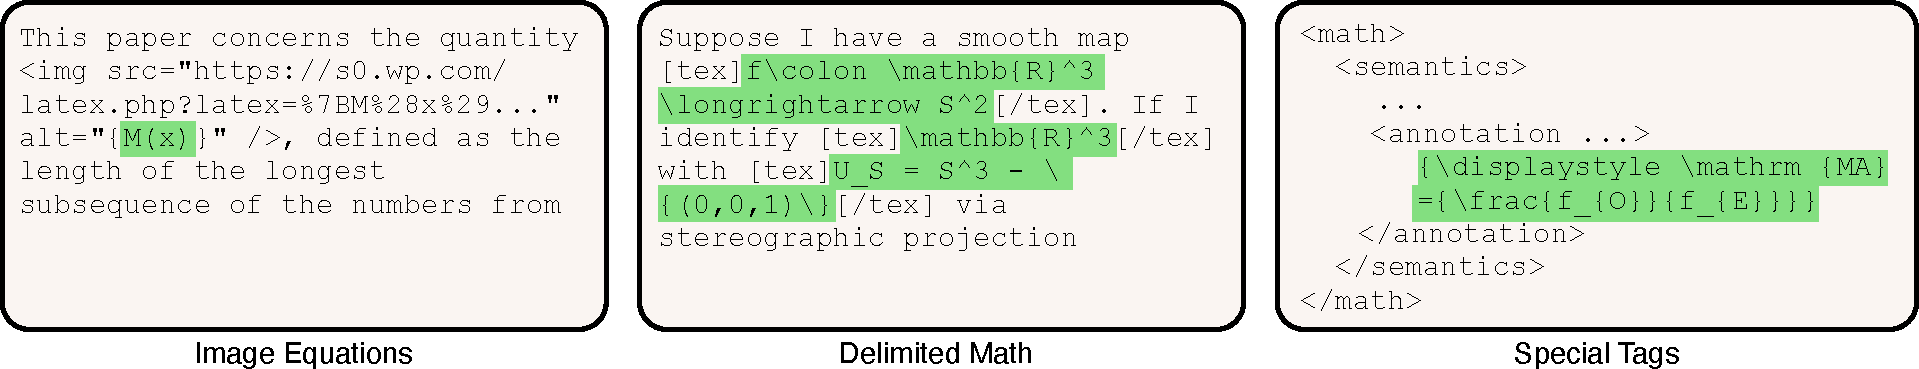
\includegraphics[width=\textwidth]{figures/latex_examples.pdf}
\end{center}
\vspace{-1.2em}
\caption{\LaTeX{} formulas can be embedded in HTML documents in many ways, including in images, within arbitrary delimiters, and within special tags. Most common text-extraction pipelines do not extract \LaTeX{} code properly.}
\end{figure}

\begin{enumerate}
    \item \texttt{equation} and \texttt{align} environments.
    \item The \texttt{alttext} of elements with special classes like \texttt{tex}.
    \item Images from domains like \texttt{latex.codecogs.com} often include equations encoded in the URL.
    \item Special wordpress plugins.
    \item \texttt{<math>} tags with \texttt{<annotation encoding="application/x-tex">} blocks within them.
    \item \texttt{<math>} tags with MathML content. We use a style sheet to convert these equations into \LaTeX{}.
    \item MathJax equations encoded in the text of the page.
\end{enumerate}

The relative frequencies of the different ways math is encoded can be found in \autoref{table:latex-types} in the appendix.

\paragraph{DOM Processing} After extracting the \LaTeX{} equations from the HTML, we do several processing steps on the DOM-tree of the HTML document. This includes removing invisible elements based on their styles, removing buttons and link clusters, annotating code, tables, and headers, and removing known problematic elements based on class or ID.

\paragraph{Text Extraction} We use the \texttt{extract\_plain\_text(main\_content=True)} method in Resiliparse \citep{bevendorff:2018} to extract the main content text from the DOM following several preprocessing steps to get around common issues with their specific implementation that cause it to be overly sensitive when removing boilerplate.

\paragraph{Line Processing} After extracting the plain text on the page using Resiliparse, we apply our own processing to remove boilerplate lines based on an iteratively-refined set of common boilerplate phrases, remove empty headers, and escape dollar signs that are not part of \LaTeX{} equations.

\subsection{Filtering}
\label{sec:filtering}

We apply filtering with the goal of removing non-English documents (since our filters pipeline is optimized for English), removing documents that are not mathematical, and removing low-quality documents that would be harmful to train a language model on. We apply the following filters in order:

\begin{figure}[t!]
\begin{center}
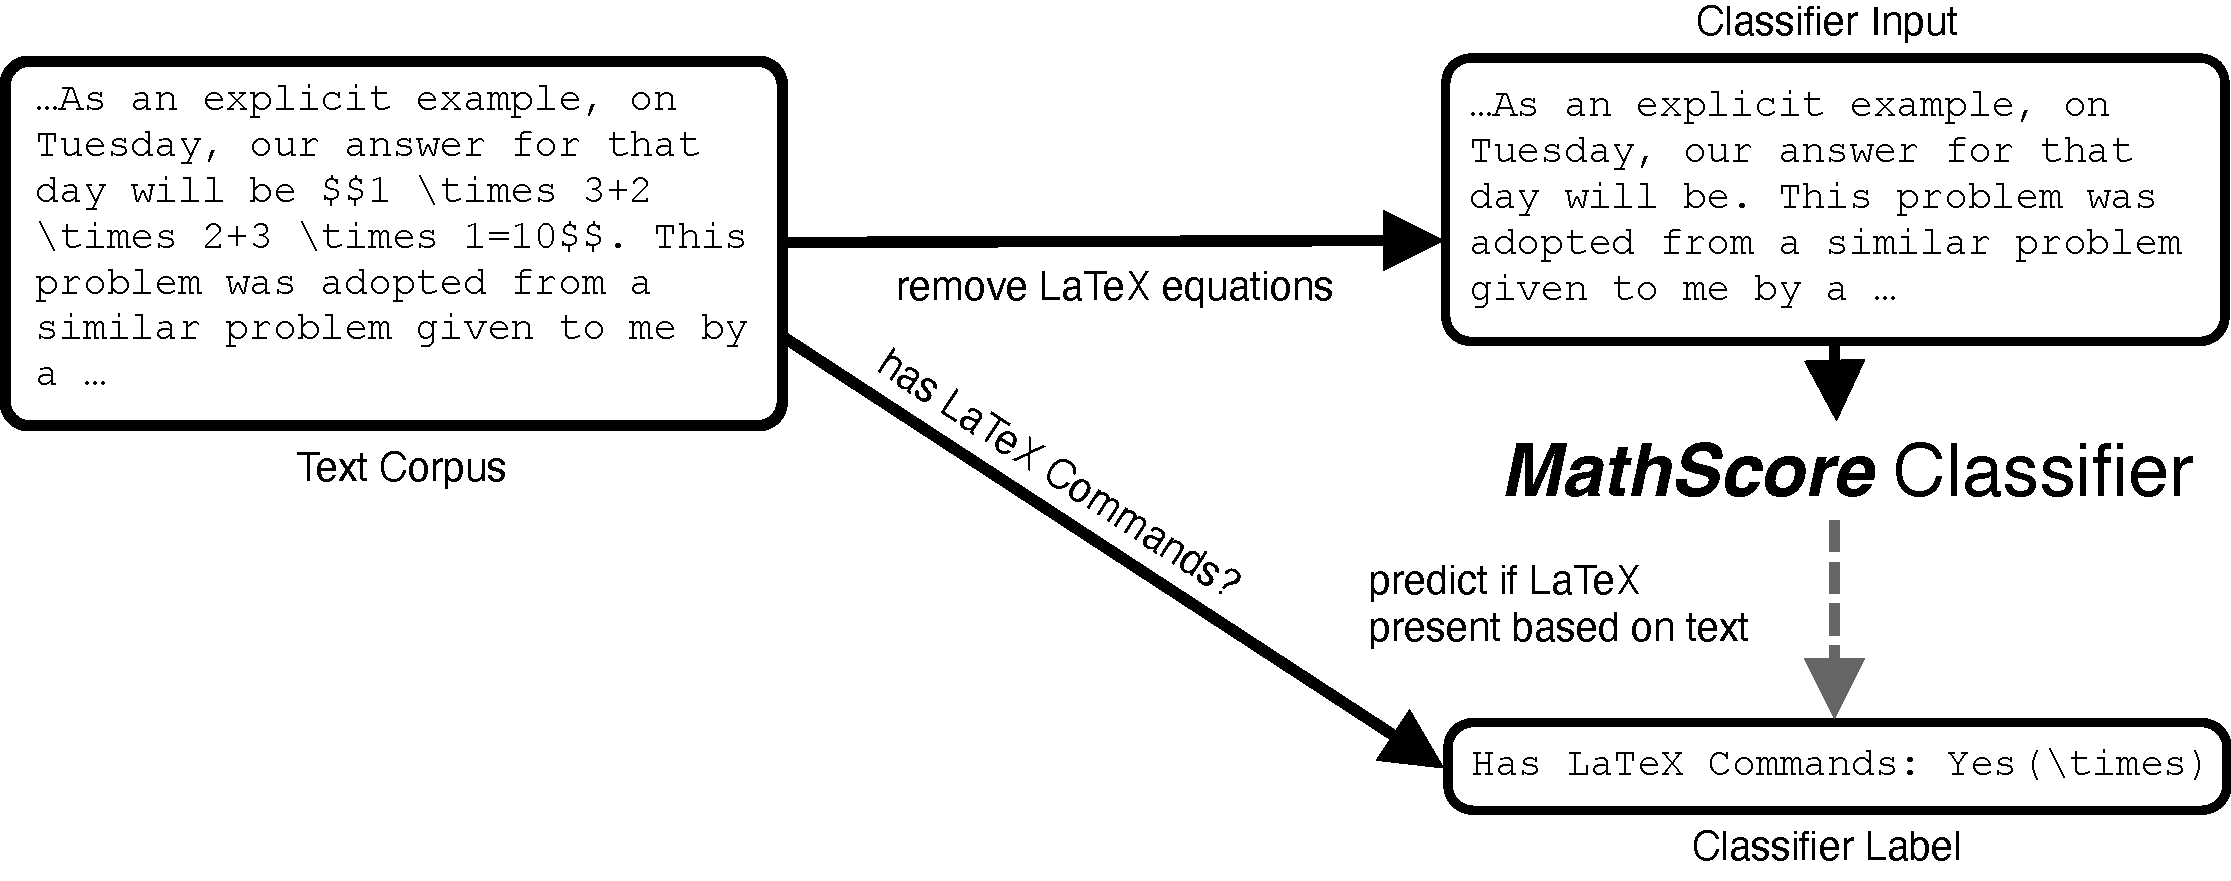
\includegraphics[width=\textwidth]{figures/MathScore.pdf}
\end{center}
\vspace{-1em}
\caption{The MathScore classifier used in filtering OpenWebMath is trained to predict whether a text has any of the most popular \LaTeX{} commands based only on surrounding words. This lets us include documents on the web that do not include extractable \LaTeX{} but still contain technical content.}
\vspace{-1em}
\label{fig:mathscore}
\end{figure}

\begin{enumerate}
    \item We use a FastText language identification model \citep{joulin2016fasttext} to remove documents that are not in English.
    \item We use our \textit{MathScore} classifier (see \autoref{sec:math_score}) to get a probability that the document is mathematical. If our previous extraction step found \LaTeX{} equations, we keep documents with a probability of over 0.17. If no \LaTeX{} equations were found, we keep documents with a probability of over 0.8.
    \item We use a KenLM language model \citep{heafield2011kenlm} trained on ProofPile \citep{azerbayev2023proofnet} to get a perplexity score for each document. We remove documents with a perplexity score of more than 15,000.
\end{enumerate}

\subsubsection{Math Score}
\label{sec:math_score}

During our filtering process, we train a model to predict the probability a document is mathematical, which we call \textit{MathScore}. We first gather a dataset of hundreds of thousands documents extracted from our pipeline from an early stage of the project, and label them depending on whether they contain one of the top-100 most common \LaTeX{} commands. We then remove any \LaTeX{} code from the documents and train a classifier to predict whether the documents contain one of these common \LaTeX{} commands. The training process for \textit{MathScore} is depicted in \autoref{fig:mathscore}. Since we remove all \LaTeX{} code from the features fed into the model, the model needs to learn the words and phrases most commonly associated with \LaTeX{} content. We use FastText \citep{joulin2016fasttext} to train this model, and find based on manual inspection that content with a score of under 0.2 is very unlikely to contain useful mathematical content.

\subsection{Deduplication}

Due to the large amount of duplicate documents in Common Crawl, we apply a deduplication step to remove near-duplicate documents. We use the SimHash implementation from text-dedup \citep{text-dedup} to deduplicate the dataset using a threshold of 0.7. We find that this threshold is high enough to remove most duplicate documents even if they have slight differences in their texts.

\subsection{Manual Inspection}

Finally, we manually inspect the top domains by document count, the top domains by character count, and the longest documents in the dataset to ensure that the documents are high quality. We remove domains that are not high quality or clearly not mathematical by adding domains to a blacklist and adding domain filters such as removing user profile pages, abstract-hosting websites as in \citet{lewkowycz2022solving}, and removing search result pages.